% DSC5002 group project -- LLNCS format (Springer), compact version
\documentclass[runningheads]{llncs}

\usepackage[T1]{fontenc}
\usepackage{newtxtext}
\usepackage[varvw]{newtxmath}
\usepackage{graphicx}
\usepackage{booktabs}
\usepackage{amsmath}
\usepackage{url}

\graphicspath{{figures/}{./}}

% tight float spacing: the layout, not the prose, was wasting the pages
\setlength{\textfloatsep}{4pt plus 1pt minus 1pt}
\setlength{\floatsep}{4pt plus 1pt minus 1pt}
\setlength{\intextsep}{4pt plus 1pt minus 1pt}
\setlength{\abovecaptionskip}{1pt}
\setlength{\belowcaptionskip}{0pt}

\begin{document}

\title{Two Clocks, One Comparison: Calendar- and Age-Anchored Views of Functional Health in China and England, 2011--2018}
\titlerunning{Two clocks, one comparison}

\author{Haonan Qi \and Hanchao Liu \and Bojun Song \and Zhengyuan Li \and Bin Liao \and Zhirui Chen}
\authorrunning{H. Qi et al.}

\institute{DSC5002 Exploratory Data Analysis and Visualization\\
Student IDs: 72640890, 72640514, 72640354, 72640157, 72640434, 72640772}

\maketitle

\begin{abstract}
Cross-national comparisons of ageing usually take the same survey year in each country and read off the gap. Because the samples differ in age composition, and that composition moves as panels age and refresh, such a mean mixes the level of limitation with the age structure. We compare the same four rounds of harmonised CHARLS (China) and ELSA (England) data, 2011--2018, on two clocks: calendar-matched rounds, and a common age axis. On the calendar clock the China--England gap in activities-of-daily-living (ADL) limitations is small and stable, $+0.07$ on a 0--5 scale. On the age clock the same data give $-0.05$ at age 50 and $+0.33$ at age 79, because ADL limitations rise about 2.3 times faster with age in China (IADL, 4.4 times), on the count scale. The readings agree only around age 55--60. Worsening is a minority event individually; the contrast survives four specifications; and for diabetes the calendar axis carries the larger signal, so the informative clock depends on the outcome.
\keywords{Ageing \and ADL \and IADL \and cross-national comparison \and CHARLS \and ELSA.}
\end{abstract}

\section{Introduction}

Difficulty bathing, dressing, shopping or managing money drives care needs and quality of life. China and England offer a clean comparison because both run HRS-family panels with harmonised instruments: CHARLS and ELSA ask the same activities-of-daily-living questions, so a difference in the answers is not a difference in the questionnaire.

Such comparisons are normally made on the \emph{calendar clock}---same year, compare means. That answers ``in 2015, how did the populations differ?'', but the populations differ in age composition, and composition moves as panels refresh. The alternative, the \emph{age clock}, compares people of the same age regardless of round and answers ``at 70, how do they differ?'', which is usually the question a care system cares about.

We ask how large the gap is on each clock, whether the age gradients differ, and how much the choice of clock changes the reader's answer. Calendar: a small, stable +0.07 ADL. Age: $-0.05$ at 50 rising to $+0.33$ at 79, because limitations rise 2.3 times faster with age in China. Reporting only one clock invites the wrong inference.

\section{Data}

\paragraph{Surveys.} CHARLS covers Chinese adults aged 45+ (spouses regardless of age) in waves 1--4 (2011, 2013, 2015, 2018). ELSA covers English adults aged 50+ in ten waves from 2002. We use the Gateway Harmonized files (D.2 and H), whose variable names and constructions are designed to be comparable across HRS-family studies.

\paragraph{Calendar matching.} CHARLS waves 1--4 define the rounds; for ELSA we take the wave whose fieldwork overlaps most closely---waves 5, 6, 7 and 9---giving an average mismatch of about 0.8 years (Fig.~\ref{fig:design}).

\begin{figure}[!htbp]
\centering
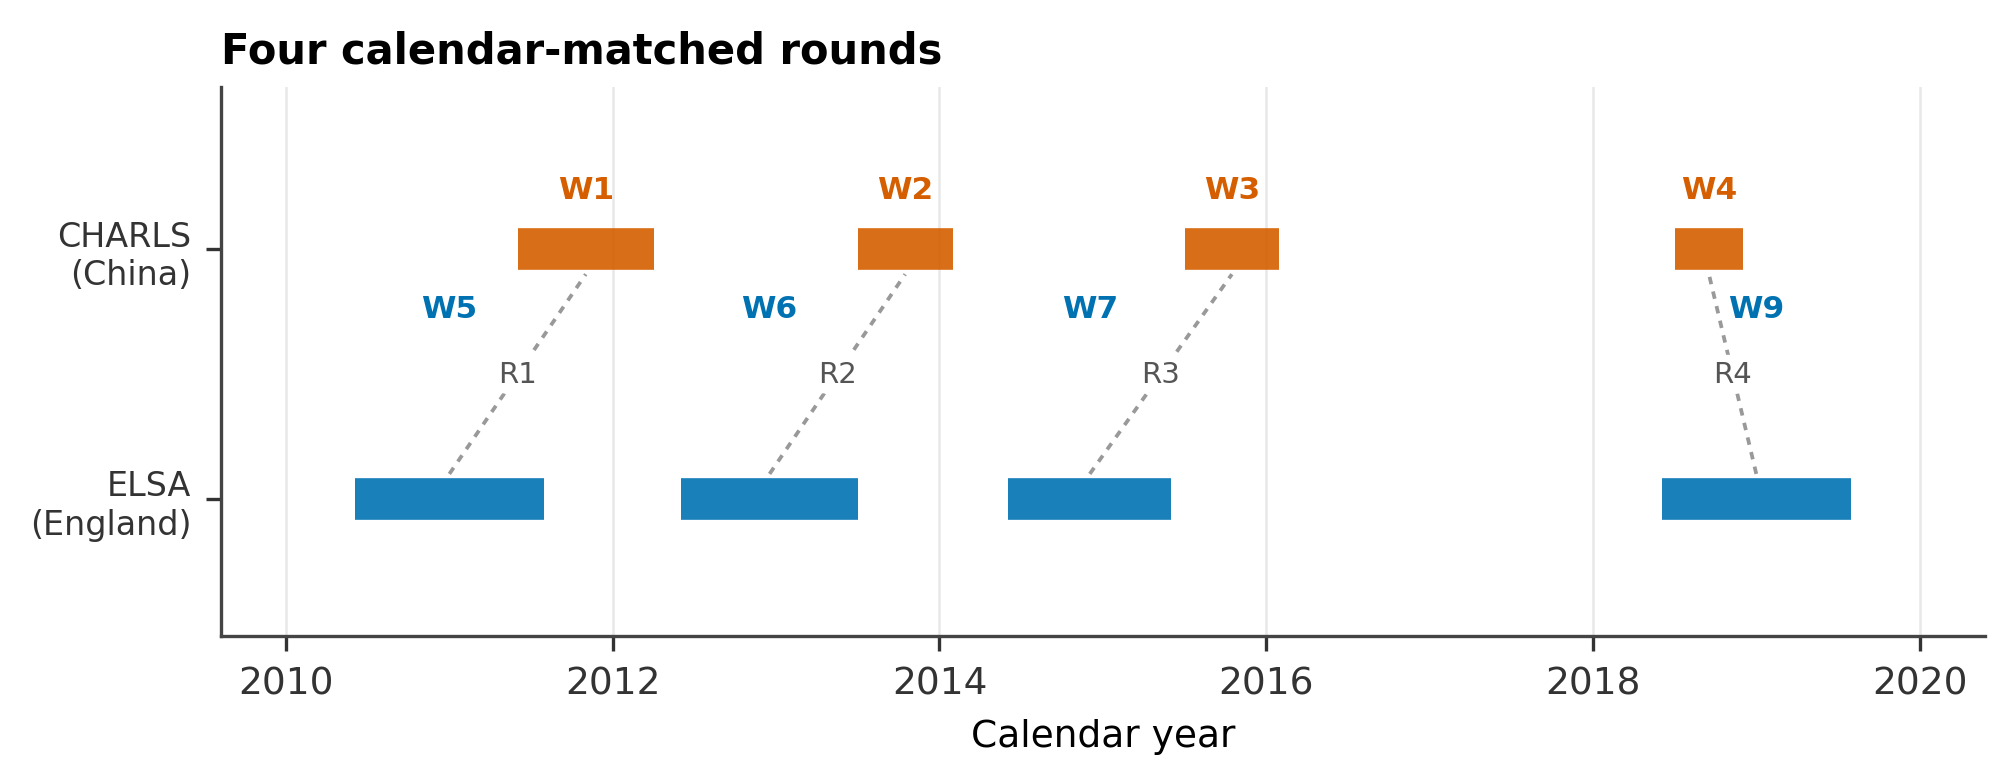
\includegraphics[width=0.86\textwidth]{F1_design.png}
\Description{Timeline pairing CHARLS waves 1 to 4 with ELSA waves 5, 6, 7 and 9.}
\caption{Calendar matching: CHARLS waves 1--4 paired with the closest ELSA wave; dashed lines join fieldwork midpoints.}
\label{fig:design}
\end{figure}

\paragraph{Instruments and sample.} The ADL count sums five activities reported as difficult (bathing, dressing, eating, getting in and out of bed, using the toilet; 0--5); the IADL count sums four (managing money, medication, shopping, preparing meals; 0--4). The codebooks confirm identical item lists. Restricting to ages 50--79 leaves 92,411 person-rounds: 59,049 from CHARLS (21,177 people) and 33,362 from ELSA (12,162), with 39\% and 37\% observed in all four rounds (Table~\ref{tab:sample}).

\begin{table}[!htbp]
\caption{Analytic sample by country and round, ages 50--79. ADL and IADL are mean counts. Unweighted.}
\label{tab:sample}
\centering
\scriptsize
\setlength{\tabcolsep}{3pt}
\begin{tabular}{llrrrrrrr}
\toprule
Round & Country & $n$ & Age & \% 65+ & \% fem. & ADL & IADL & \% tert. \\
\midrule
2011 & China   & 13,008 & 61.3 & 31 & 50 & 0.35 & 0.40 & 1.8 \\
2013 & China   & 14,213 & 61.4 & 32 & 50 & 0.33 & 0.33 & 1.8 \\
2015 & China   & 15,650 & 61.6 & 34 & 51 & 0.39 & 0.35 & 1.9 \\
2018 & China   & 16,178 & 62.1 & 39 & 52 & 0.36 & 0.36 & 1.9 \\
2011 & England &  8,859 & 64.6 & 47 & 55 & 0.29 & 0.14 & 17.8 \\
2013 & England &  9,102 & 64.5 & 48 & 54 & 0.29 & 0.15 & 19.1 \\
2015 & England &  8,227 & 65.1 & 53 & 55 & 0.27 & 0.14 & 19.6 \\
2018 & England &  7,174 & 65.2 & 56 & 55 & 0.28 & 0.15 & 22.2 \\
\bottomrule
\end{tabular}
\end{table}

\paragraph{What we dropped.} Self-rated health is not fielded in CHARLS wave 4, so a four-round comparison is impossible. Immediate word recall breaks in wave 4: mean recall falls 0.4--0.9 words \emph{within every age band} (4.35 $\rightarrow$ 3.81 at ages 50--54) while ELSA is flat---a break larger than the entire age gradient, consistent with a change in test administration. Using it would have measured the instrument, not ageing.

\section{Methods}

\paragraph{Axis A, calendar anchoring.} Mean counts per country and round with 95\% intervals, plus the age mix and respondent flow behind them.

\paragraph{Axis B, age anchoring.} We regress the outcome on age, centred at 65, with round fixed effects, separately by country:
\begin{equation}
y_{ir} = \alpha + \beta\,(\text{age}_{ir} - 65) + \gamma_r + \varepsilon_{ir}.
\end{equation}
The round effects absorb any common calendar shift, so $\beta$ comes from differences between people of different ages in the same round; standard errors are clustered on the person. A pooled model with an age $\times$ country interaction tests whether the gradients differ.

\paragraph{Gap curve and robustness.} From the pooled model we predict the gap at every age from 50 to 79, averaging over rounds and simulating 2,000 draws for 95\% intervals. Four specifications follow: the main model; dropping round 1 (CHARLS wave-1 IADL runs about 0.06 high); adding the harmonised education indicator; and person fixed effects, which remove all time-invariant differences between people. We also re-estimate with a Poisson link for the count and a logit for any limitation.

\paragraph{Inference.} Estimates are unweighted and describe the samples, not the national populations.

\section{Results}

\subsection{The Calendar Clock}

Neither country moves much (Fig.~\ref{fig:calendar}): ADL limitations average 0.35 in China and 0.29 in England in 2011, and 0.36 and 0.28 in 2018; IADL averages 0.40 and 0.14, then 0.36 and 0.15. The gap averages $+0.072$ ADL and $+0.216$ IADL points, varying by about 0.03 across rounds: older Chinese adults report somewhat more limitation, and the gap looks stable.

\begin{figure}[!htbp]
\centering
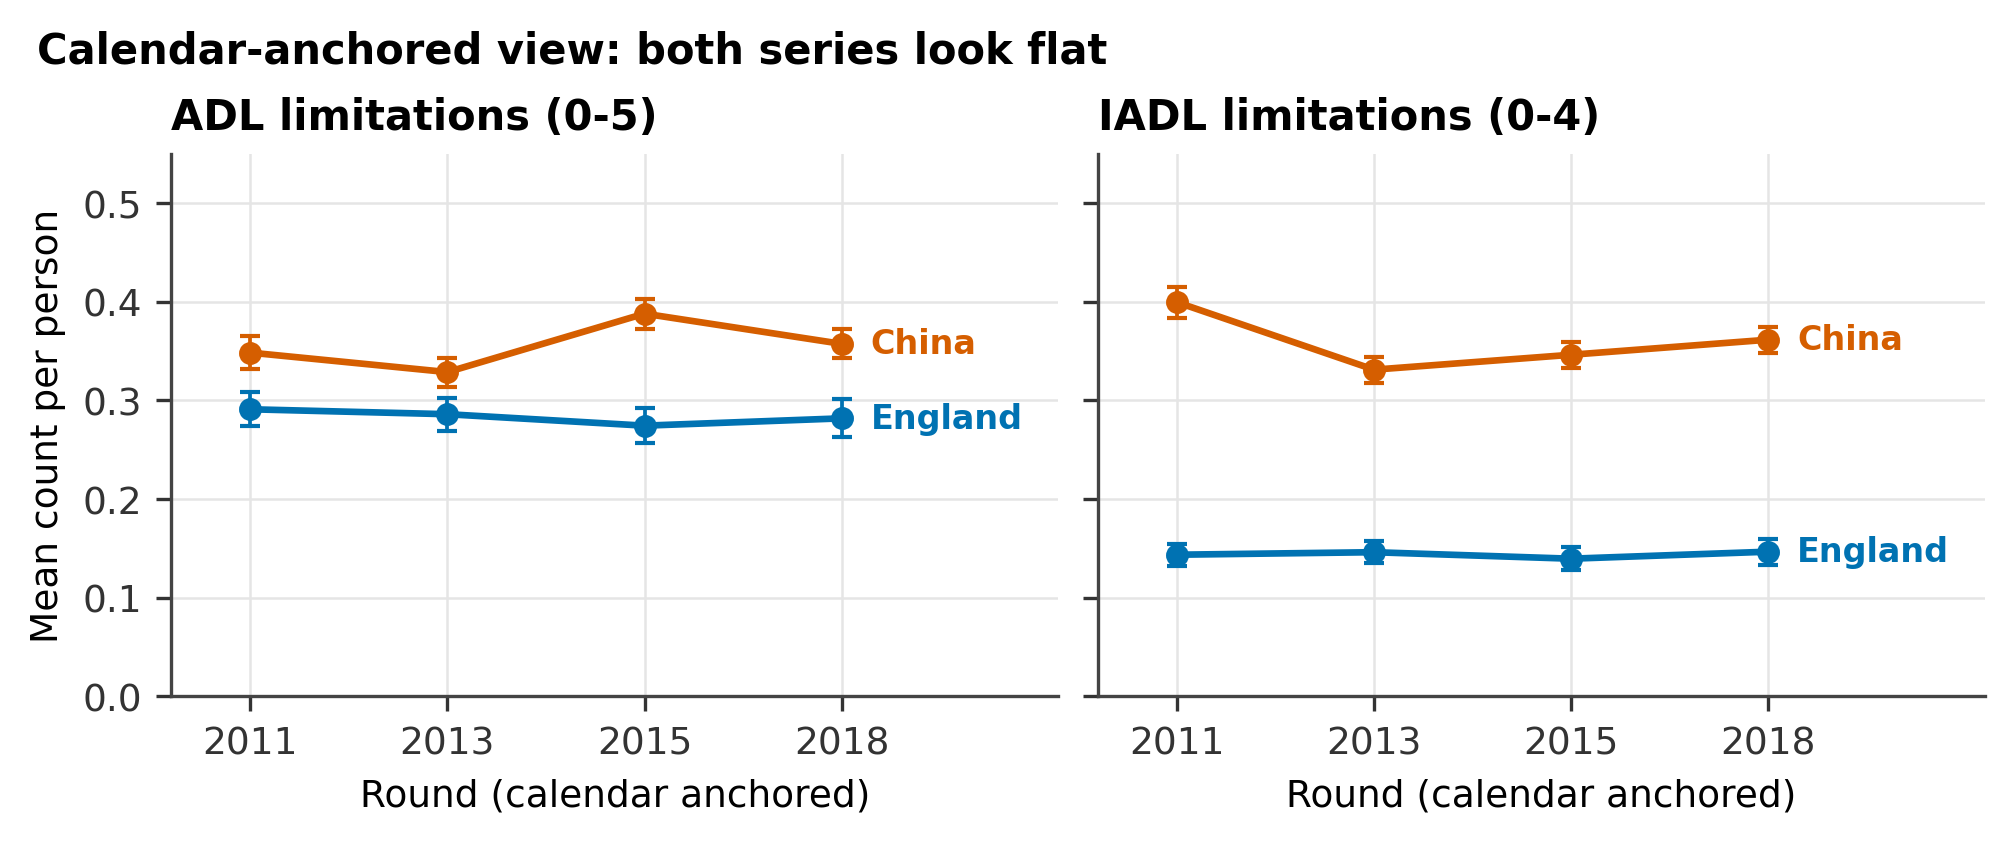
\includegraphics[width=0.86\textwidth]{F2_calendar_anchored.png}
\Description{Mean ADL and IADL limitations by round for China and England, both nearly flat.}
\caption{Calendar-anchored means (95\% intervals): both series flat, gap small.}
\label{fig:calendar}
\end{figure}

The stability is an artefact of composition (Fig.~\ref{fig:comp}). In 2011 the Chinese sample is already 3.4 years younger (61.3 vs 64.6) and 31\% rather than 47\% is aged 65+. Refreshment then moves both: the 65+ share rises from 0.31 to 0.39 in China and 0.47 to 0.56 in England, and within the fixed 2011 cohort the rise is steeper (0.31 $\rightarrow$ 0.57; 0.47 $\rightarrow$ 0.81). The cohort's mean age rises only about five years over seven of fieldwork, so older respondents left faster. China adds 3,000--3,300 per round against 1,900--2,500 losses; England's losses overtake refreshment from 2015. Ageing and replacement happen at once, and the flat series are their net.

\begin{figure}[!htbp]
\centering
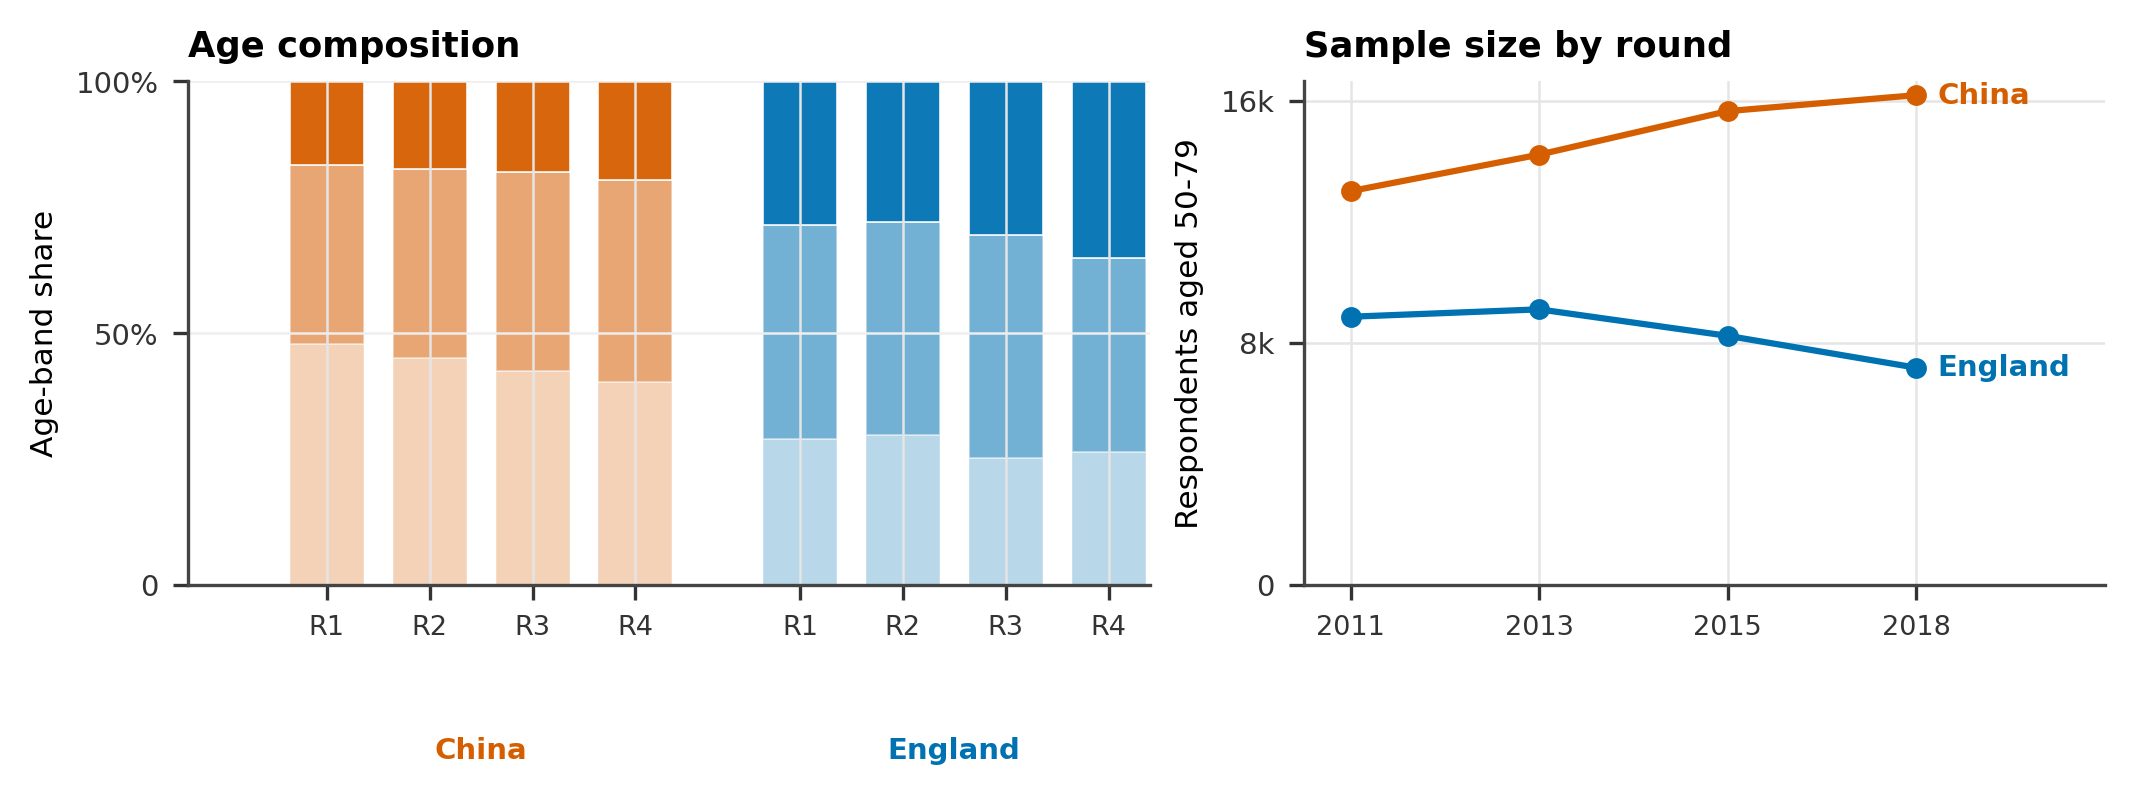
\includegraphics[width=0.90\textwidth]{figC_composition_flow.png}
\Description{Left: age-band composition by round. Right: number of respondents by round for both countries.}
\caption{Composition and sample flow: age-band shares by round (left), respondents per round (right).}
\label{fig:comp}
\end{figure}

\subsection{The Age Clock}

At 50--54 the countries are close (ADL 0.17 vs 0.19; IADL 0.19 vs 0.11) and then separate (Fig.~\ref{fig:age}). The ADL slope is 0.0221 per year in China (95\% CI 0.0207--0.0235), or $+0.22$ per decade, against 0.0094 (0.0078--0.0110), or $+0.09$, in England; the interaction is $-0.0128$ (SE 0.0011, $p<0.001$). On the count scale the Chinese gradient is 2.3 times steeper. IADL is sharper still (Table~\ref{tab:slopes}): 0.0207 against 0.0047, a ratio of 4.4, interaction $-0.0159$ (SE 0.0009). In England IADL barely rises across the range (0.07 to 0.21); in China it roughly quadruples.

\begin{figure}[!htbp]
\centering
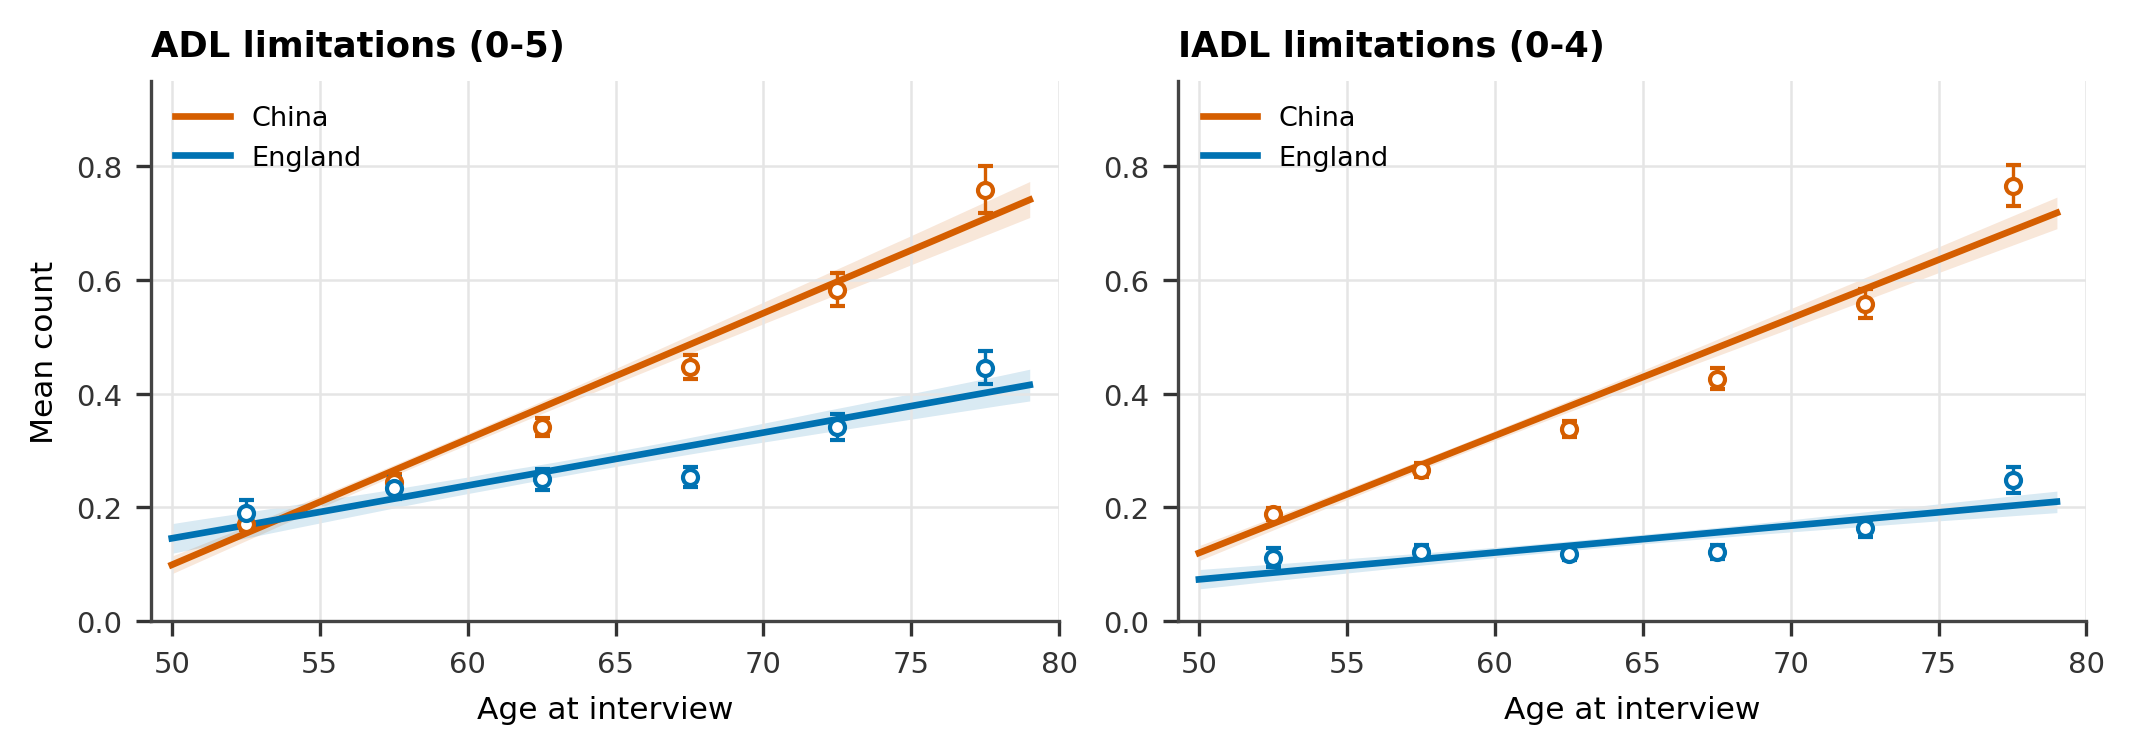
\includegraphics[width=0.90\textwidth]{figD_age_curves.png}
\Description{Binned means and fitted age gradients for ADL and IADL in both countries.}
\caption{Age-anchored view: 5-year bin means (95\% CI) and fitted gradients (95\% bands); ADL lines cross near 54.}
\label{fig:age}
\end{figure}

\begin{table}[!htbp]
\caption{Age slopes (round fixed effects, person-clustered SEs). Difference is the age $\times$ country interaction from the pooled model.}
\label{tab:slopes}
\centering
\scriptsize
\setlength{\tabcolsep}{4pt}
\begin{tabular}{llrccl}
\toprule
Outcome & Group & Slope/year & 95\% CI & Per decade & $p$ \\
\midrule
ADL (0--5)   & China      & 0.0221  & 0.0207, 0.0235 & 0.22  & \\
             & England    & 0.0094  & 0.0078, 0.0110 & 0.09  & \\
             & Difference & $-0.0128$ & $-0.0149$, $-0.0107$ & $-0.13$ & $<0.001$ \\
IADL (0--4)  & China      & 0.0207  & 0.0194, 0.0219 & 0.21  & \\
             & England    & 0.0047  & 0.0036, 0.0058 & 0.05  & \\
             & Difference & $-0.0159$ & $-0.0176$, $-0.0142$ & $-0.16$ & $<0.001$ \\
\bottomrule
\end{tabular}
\end{table}

\subsection{What the Clock Changes}

Figure~\ref{fig:gap} puts both readings on one axis. The flat dashed line is the unadjusted calendar gap ($+0.07$). The rising curve is the gap at each age: $-0.05$ at 50 (China significantly \emph{lower}, CI $-0.08$ to $-0.02$), indistinguishable from zero at 55 ($+0.02$), $+0.15$ at 65 and $+0.33$ at 79. The two agree only around 55--60; at either end the calendar number is wrong by a factor of two to seven. For IADL the calendar gap ($+0.22$) understates the age-65 ($+0.28$) and age-79 ($+0.51$) gaps, and there is no crossover: China is higher at every age, by a widening margin.

\begin{figure}[!htbp]
\centering
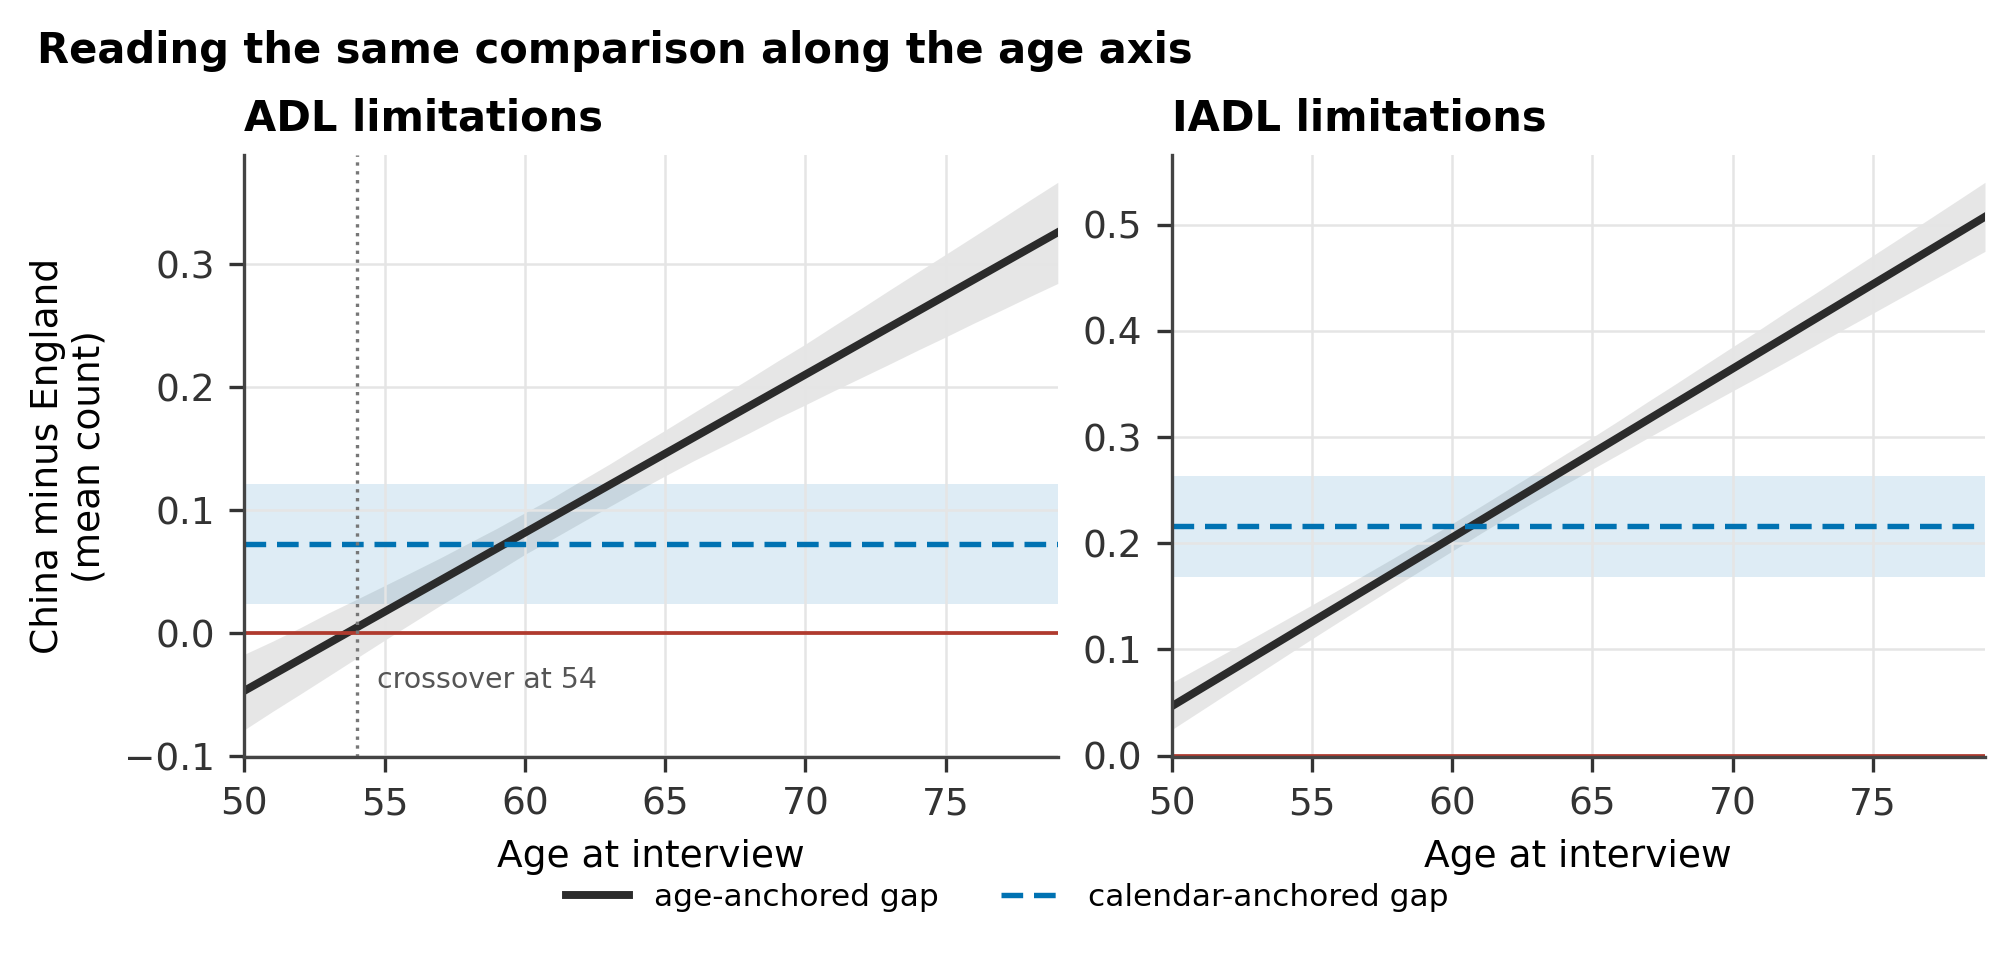
\includegraphics[width=0.86\textwidth]{F7_gap_by_age.png}
\Description{China-minus-England gap by age as a rising curve, with the flat calendar gap as reference.}
\caption{Both readings on one axis: the predicted gap by age (curve) and the unadjusted calendar gap (dashed).}
\label{fig:gap}
\end{figure}

\subsection{Who Actually Changes}

A gradient summarises many histories, and most contain no change (Fig.~\ref{fig:within}). Between consecutive rounds the ADL count rose for 12.9\%, 15.5\% and 12.7\% of Chinese respondents, against 9.3\%, 8.8\% and 10.5\% in England. Over seven years, 18\% of Chinese and 12\% of English respondents present in both rounds reported more limitations, while 73\% and 82\% reported exactly the same count. The country difference is not that everyone in China deteriorates faster; it is that the minority who do is larger, and compounds with age.

\begin{figure}[!htbp]
\centering
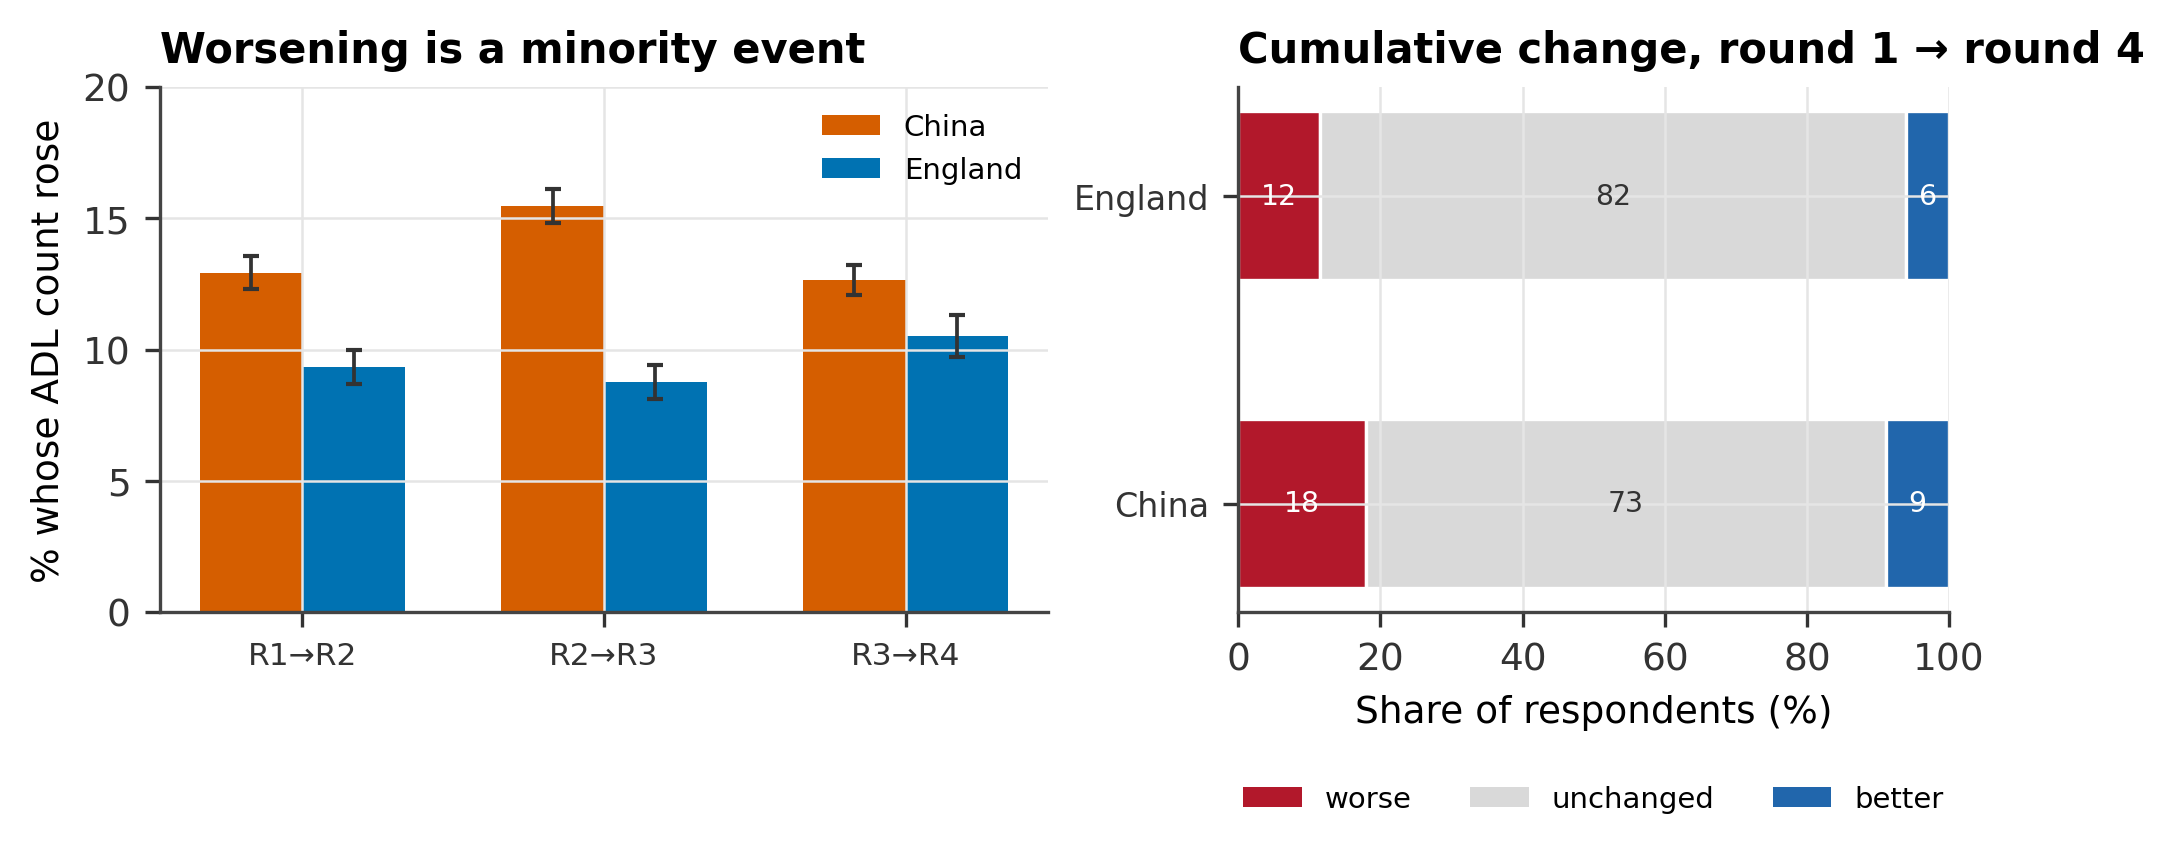
\includegraphics[width=0.86\textwidth]{F8_within_person.png}
\Description{Share worsening between rounds, and cumulative change from round 1 to round 4.}
\caption{Within-person change: share worsening between rounds (left), cumulative change 1$\rightarrow$4 (right).}
\label{fig:within}
\end{figure}

\subsection{Robustness}

Figure~\ref{fig:robust} reports four specifications. Dropping round 1 gives 0.0222 vs 0.0087 for ADL; adding education leaves China almost unchanged (0.0213) and lowers England (0.0068); person fixed effects raise both (0.0334 vs 0.0139) while the ratio stays at 2.4. IADL gives 0.0202/0.0043, 0.0196/0.0027 and 0.0210/0.0095. Because 82--85\% report zero limitations, we also re-estimated with a Poisson link and a logit for any limitation. The ordering and significance hold ($p<0.001$ throughout) but the multiplier shrinks: for ADL it is 2.36 (1.93--2.79) on the count scale, 1.77 (1.44--2.09) in log-rate terms and 1.35 (1.17--1.53) in log-odds terms; for IADL, 4.39, 1.66 and 1.87. The direction is robust; the headline multiplier is scale-specific.

\begin{figure}[!htbp]
\centering
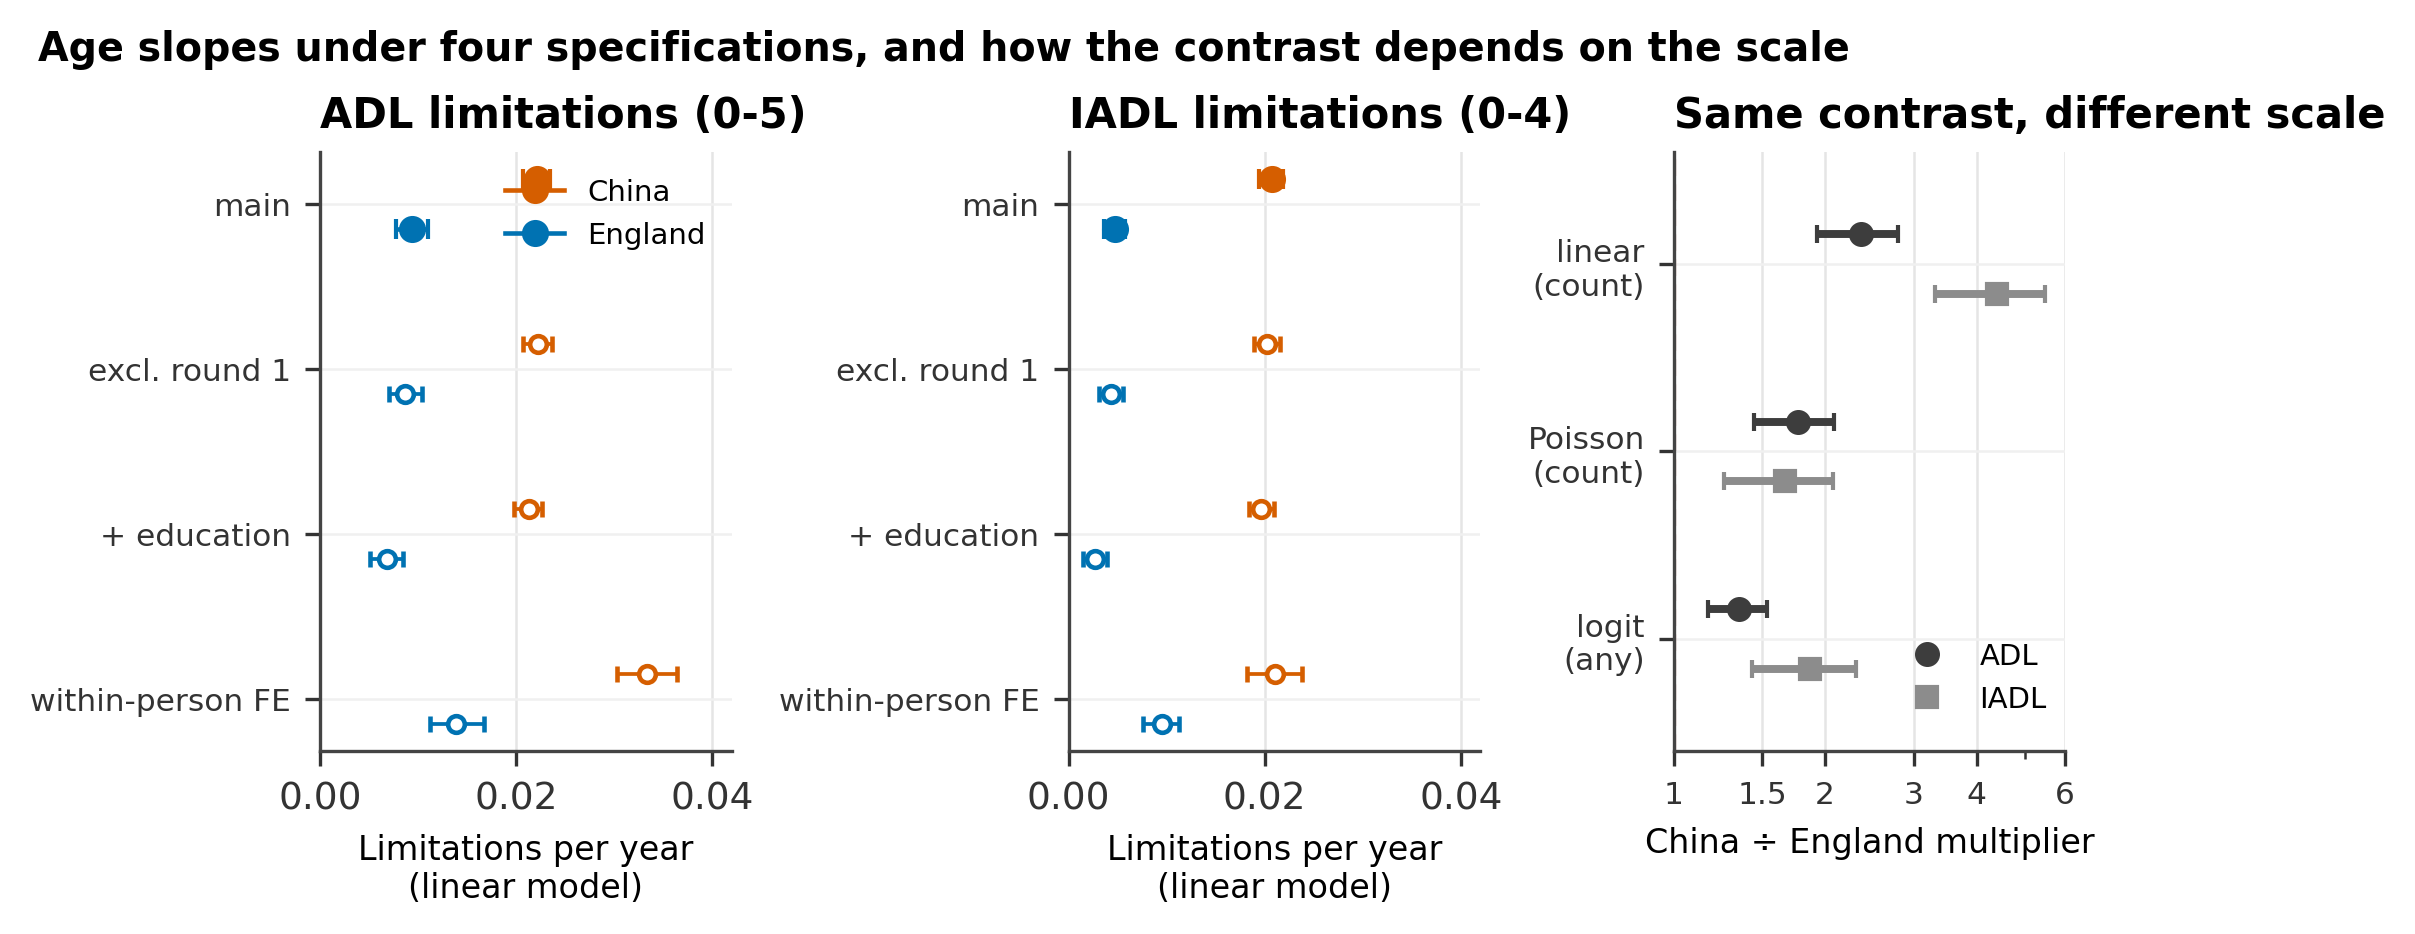
\includegraphics[width=0.86\textwidth]{F9_slope_robustness.png}
\Description{Slopes under four specifications and the country multiplier under three link functions.}
\caption{Robustness: slopes under four specifications (left, centre) and the China-to-England multiplier under three link functions (right).}
\label{fig:robust}
\end{figure}

\subsection{A Counter-Example}

Not every outcome behaves this way (Fig.~\ref{fig:diabetes}). English diabetes prevalence rises steadily from 5.7\% at 50--54 to 15.4\% at 75--79, whereas Chinese prevalence climbs to about 12\% at 65--69 and then flattens and falls. On the calendar axis, age-standardised prevalence rises from 7.0\% to 13.3\% in China---nearly doubling---against 9.3\% to 11.5\% in England. Here the calendar axis carries the signal and the age axis is ambiguous, so which clock is informative depends on the outcome, and a report should say which it is using. We cannot separate incidence from improved diagnosis: the item records whether a doctor ever said the respondent had diabetes.

\begin{figure}[!htbp]
\centering
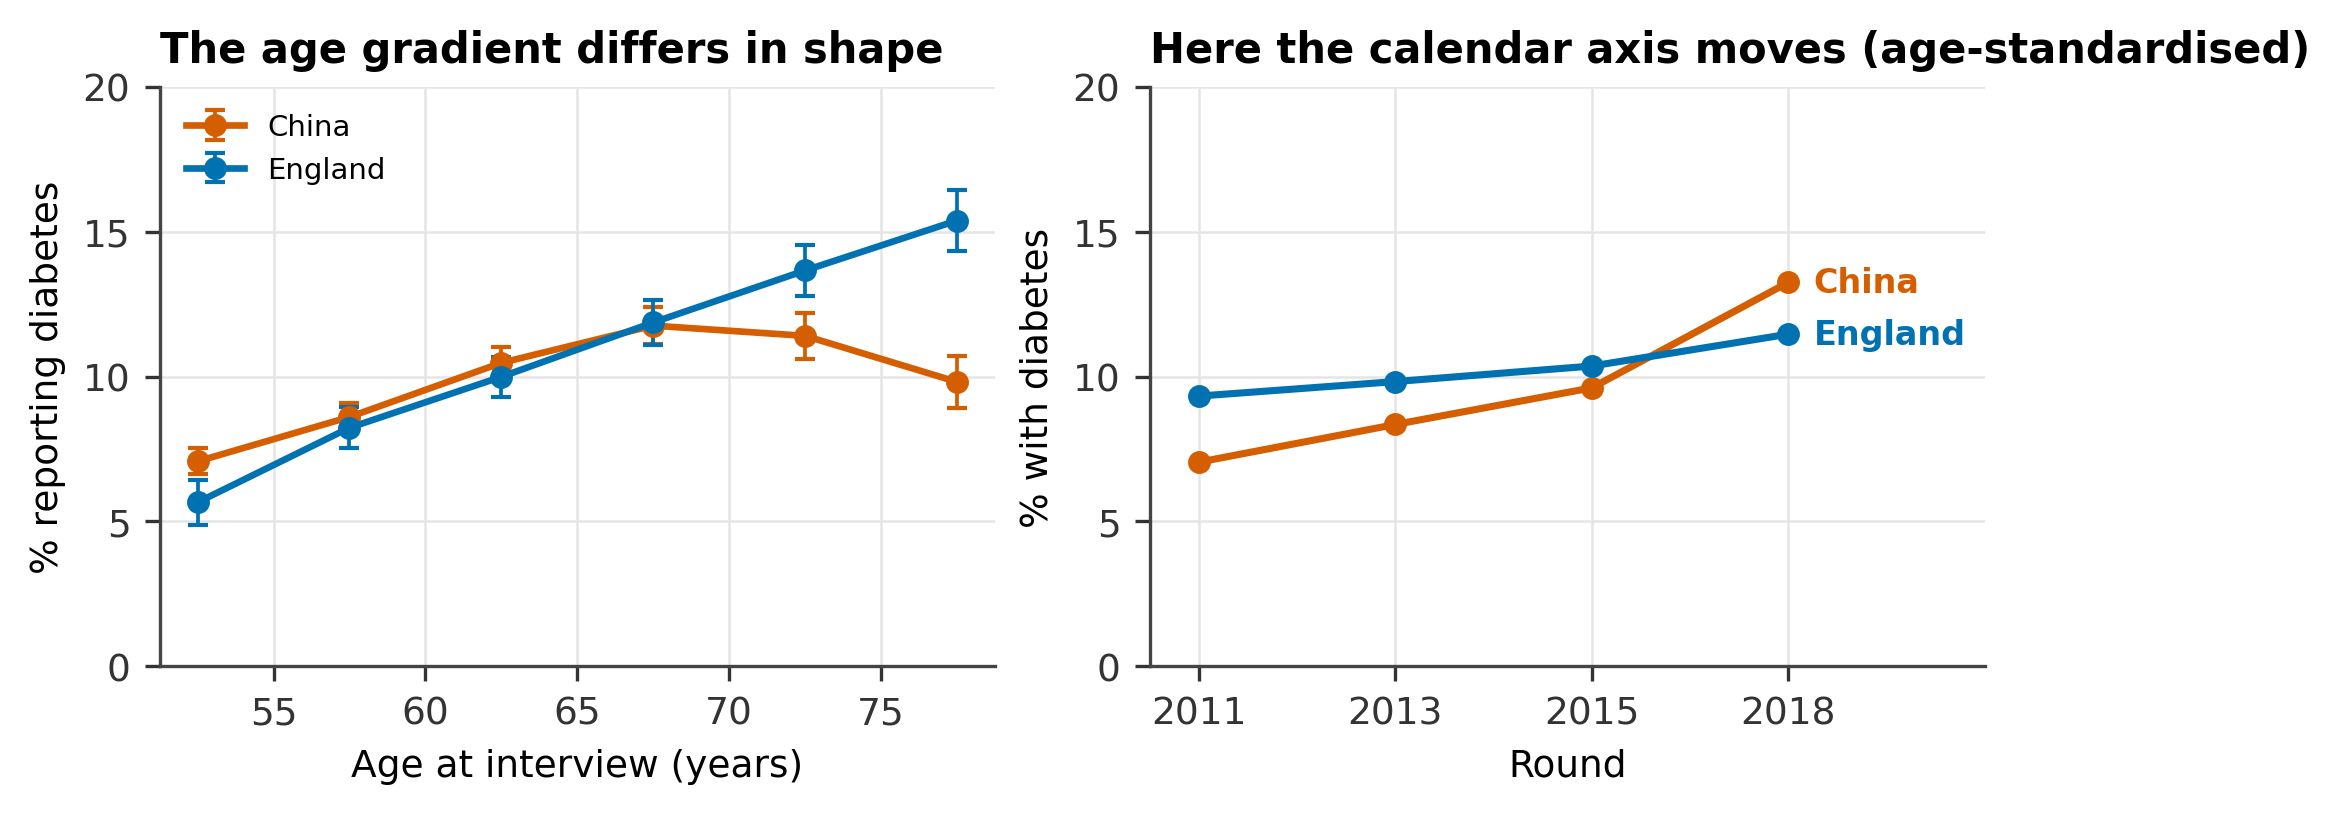
\includegraphics[width=0.86\textwidth]{F10_diabetes.png}
\Description{Diabetes prevalence by age, and age-standardised prevalence by round.}
\caption{A different outcome: diabetes prevalence by age (left) and age-standardised by round (right).}
\label{fig:diabetes}
\end{figure}

\section{Discussion}

\paragraph{Principal finding.} The two anchorings answer different questions, and the answers differ by a factor of two to seven depending on where on the age axis one looks. The calendar comparison understates the age-specific disadvantage of older Chinese adults because the Chinese sample is younger; conversely, a calendar-year gap cannot serve as a planning number for care need.

\paragraph{Why the Chinese gradient is steeper.} Four candidates, none settled here. \emph{Cohort composition}: Chinese cohorts born in the 1930s--40s had far less schooling (1.8--1.9\% tertiary against 17.8--22.2\%); adjusting for it shrinks the English gradient but barely moves China's, so education as measured is not the explanation, though it is a weak proxy for early-life conditions. \emph{Selective survival}: if high-risk Chinese adults die earlier, survivors look healthier and the slope is biased \emph{downwards}---the observed slope is steeper despite that, which strengthens the finding. \emph{Measurement}: self-reported difficulty is filtered through expectation and adaptation, and we have no anchoring vignettes; this is the largest threat to the comparison. \emph{Care environment}: adaptations may delay limitation in England, but we measure none of it, so this stays a hypothesis.

\paragraph{The crossover matters.} Chinese respondents aged 50--54 report slightly \emph{fewer} ADL limitations than English respondents of the same age; the disadvantage emerges only after about 55. ``Older adults in China are more disabled'' is therefore age-specific: at 52 it is false.

\paragraph{Limitations.} The cross-sectional gradient confounds age with cohort; person fixed effects address the cohort but introduce attrition selection. Estimates are unweighted. Outcomes are self-reported and item functioning across cultures is untested. The multiplier depends on the scale, so it should be quoted with one. Two countries and four rounds are not a general claim about developing and developed settings.

\section{Conclusion}

Asking the same question on two clocks gives two numbers, and neither is wrong. Between 2011 and 2018, ADL limitations rose about 2.3 times faster with age in China than in England on the count scale (IADL, 4.4 times), crossing over near age 54, so that a calendar-year gap of 0.07 conceals an age-specific gap running from $-0.05$ at 50 to $+0.33$ at 79. Most individuals in both countries did not change; the countries differ in the size of the minority who did. Read cross-national ageing statistics by asking which clock they were measured on.

\begin{credits}
\subsubsection{\ackname}
This work uses data from the Gateway to Global Aging Data harmonised CHARLS and ELSA files, and was carried out as a group project for DSC5002 Exploratory Data Analysis and Visualization.

\subsubsection{\discintname}
Generative AI was used to draft analysis code and to help structure the manuscript. All data handling, variable definitions, model specifications and reported numbers were checked against the codebooks and re-computed from the harmonised files; the figures are reproduced by the archived scripts. The authors have no competing interests to declare.

\subsubsection{Author contributions.}
All six members contributed to the design, interpretation and revision of the study and approved the final version. Specific contributions: Haonan Qi, research question and manuscript; Hanchao Liu and Bojun Song, data extraction and variable checks; Zhengyuan Li, models and robustness; Bin Liao, tables; Zhirui Chen, figures and presentation.
\end{credits}

\begin{thebibliography}{8}

\bibitem{ref_charls}
Zhao, Y., Hu, Y., Smith, J.P., Strauss, J., Yang, G.: Cohort profile: the China Health and Retirement Longitudinal Study (CHARLS). International Journal of Epidemiology \textbf{43}(1), 61--68 (2014)

\bibitem{ref_elsa}
Steptoe, A., Breeze, E., Banks, J., Nazroo, J.: Cohort profile: the English Longitudinal Study of Ageing. International Journal of Epidemiology \textbf{42}(6), 1640--1648 (2013)

\bibitem{ref_gateway}
Gateway to Global Aging Data: Harmonized CHARLS Documentation, Version D.2; Harmonized ELSA Documentation, Version H. University of Southern California

\bibitem{ref_katz}
Katz, S., Ford, A.B., Moskowitz, R.W., Jackson, B.A., Jaffe, M.W.: Studies of illness in the aged: the index of ADL. JAMA \textbf{185}, 914--919 (1963)

\bibitem{ref_lawton}
Lawton, M.P., Brody, E.M.: Assessment of older people: self-maintaining and instrumental activities of daily living. The Gerontologist \textbf{9}(3), 179--186 (1969)

\end{thebibliography}

\end{document}
